\section{Application Scenarios}
\label{sec:scenarios}
%
We next demonstrate our obstruction-free lens via five use-cases considering scalar density volumes from baggage inspection, 3D flow simulation, radiology, air traffic planning, and diffusion tensor imaging.

\subsection{Baggage inspection: An unusual blunt object}
\label{sec:baggage}
%
In airports, security agents deal with volumetric data exploration during baggage inspections. While automatic systems can detect densities of harmful substances such as C-4, TNT, and nitroglycerin, or prohibited articles (threats) like classical firearms and knives, unusual threats are hard to find. Four main concealment strategies exist\,\cite{7819413}:

\vspace{0.15cm}
\noindent\textbf{Superposition}: A threat may be sheltered among dense materials. While possible to see through such a `shield' using high penetration (enhanced X-ray power) or image processing (contrast improvement), such techniques are not universally available and also require fine-tuning many parameters, which slows down inspection.

\vspace{0.15cm}
\noindent\textbf{Location}: Objects located in the corners, edges, or in the luggage'��s frame are very hard to spot.

\vspace{0.15cm}
\noindent\textbf{Dissociation}: One can conceal a threat by spreading its parts in the luggage, \emph{e.g}, by disassembling a weapon and scattering its parts.

\vspace{0.15cm}
\noindent\textbf{Lure}: A minor threat (lure) like a small scissors is clearly visible and catch the security agent's attention who can miss the real threat.

Baggage labeled as suspicious by human inspection or automated scan heuristics must be checked by human agents. Besides time-consuming physical unpacking, one can use `virtual unpacking' tools that segment the 3D scan by a density-based confidence measure and next move the segmented objects away by animation to reduce occlusion\,\cite{Li:2012:LVV:2425296.2425325}. Such systems have been patented and used in production\,\cite{patent}. However, when the automatic segmentation is not optimal, the user must manually change its parameters, repeat the segmentation and animation, which goes back to being time consuming.

Consider the baggage scan in \autoref{f:baggage_lens} ($283 \times 189 \times 344$ voxels, dataset obtained from an actual airport scan). Automatic baggage inspection systems will not detect anything suspect here. However, while visually exploring this baggage from different angles (\autoref{f:baggage_lens}a-c), we see an object hidden between a set of mugs. To reduce occlusion, a common solution in baggage inspection is to filter materials by density in order to show or hide subsets of the volume. However, for our dataset, the suspect target has almost the same density as the surrounding mugs, so removing the latter also removes the target (\autoref{f:baggage_lens}d-f). Using the obstruction-free fish-eye lens helps here: Clicking on the sharp detail visible in \autoref{f:baggage_lens}c first gathers rays so they pass through the low-density zone between the mugs (\autoref{f:baggage_lens}f). The animation that opens the lens 
(\autoref{f:baggage_lens}e-g) reveals an unobstructed view of the target. However, this shows only a small part of the target. Scattering rays next fully reveals the target (\autoref{f:baggage_lens}h). Adjusting the lens size shows a more detailed view of the target (\autoref{f:baggage_lens}i). Next, locally turning the viewpoint around the target (\autoref{f:rotation}) allows the agent to decide that the target is a shuriken (Japanese ninja star weapon). Since the object is very thick and blunt (see \autoref{f:rotation}), it is not an actual weapon, thus not a threat.

We evaluated our lens for this use-case by a user study. Eight airport security specialists were recruited (ages 23 to 43; experience in baggage scanning 8 months to 20 years; average familiarity with 3D tools, none considering him/herself an expert, see Fig.~\ref{fig:questanswers}).
All attended a 20-minute global demo of the lens operation. Next, they were given each a personal training session for using the tool (5 minutes), in which they were instructed on the mouse and keyboard controls. After this, they were asked to work in pairs to examine the above-mentioned baggage CT dataset to form a decision on the nature of the ninja star possible threat (20 minutes of tool usage per person, after which the pair was changed). The idea behind this is that one person operates the tool while the other poses questions or suggest explorations, much like typical airport security operators work with a scanner. At the end, they all separately filled in a web questionnaire covering several questions and also provided open feedback (questionnaire available in supplementary material). 

Figure.~\ref{fig:questanswers} shows the answers. The first question-set (S1) regarded how easy-to-use, generally effective, and effective \emph{vs} other known tools our lens is for \emph{untargeted} inspection, \emph{i.e.}, when no suspect target is partially visible. Here and next, other tools denote classical 2D X-ray or 3D CT scans used in baggage scanning that the subjects know. As Fig.~\ref{fig:questanswers}c-e shows, 
the answers (on a 5-point Likert scale) were predominantly positive: The tool is easy to use, is useful, and is actually more useful than known tools 
for untargeted exploration. The second question-set (S2) regarded how good our tool is to examine \emph{specific} targets which are partially visible. Here again, the answers were predominantly positive (Fig.~\ref{fig:questanswers}f-h). The main appreciated features of our tool are listed in Fig.~\ref{fig:questanswers}i.


\begin{figure}[htbp!]
\centering
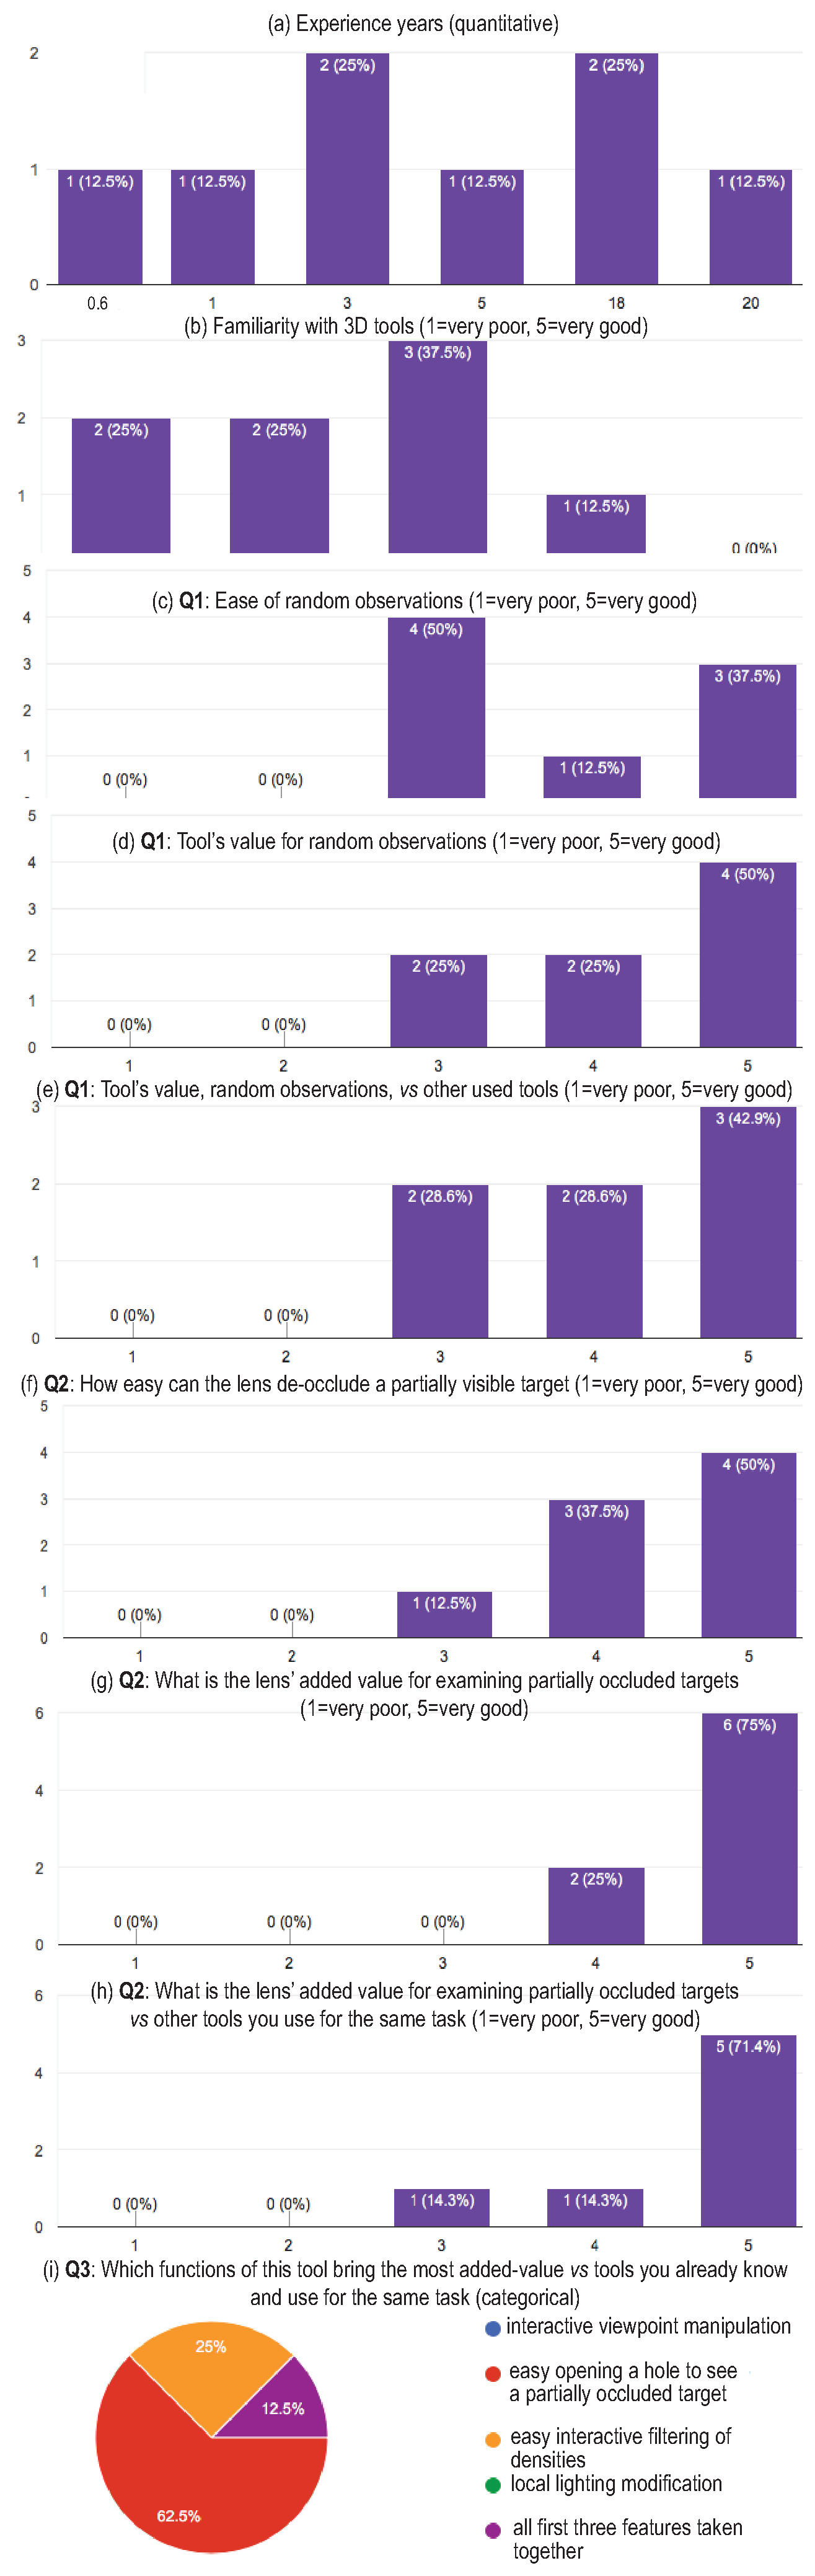
\includegraphics [width=0.42\textwidth]{images/questanswers.eps}
\vspace{-0.15cm}
\caption{Evaluation of lens-based baggage inspection (Sec.~\ref{sec:baggage}).}
\vspace{-0.15cm}
\label{fig:questanswers}
\end{figure}

We next summarize the received open feedback. According to the subjects, our tool can provide them a better perception of the items inside the baggage as compared to the classical 2D single-viewpoint X-ray machinery they routinely use. However, our tool should not be used for the typical carry-on baggage inspection which has a very small allowed inspection time (15 to 20 seconds). Our tool is much more interesting for inspecting checked-in baggage, where inspection time-windows are up to 3 minutes. The perceivedadded value for this use-case is also higher: Opening up checked-in baggage for manual inspection is much more complicated and time-consuming than for carry-on baggage. Moreover, the only system for inspecting checked-in baggage that the subjects knew of is a scanner that aims to \emph{automatically} detect threats via X-ray imagery; this system suffers from false positives, so a manual examination tool like ours could quickly eliminate such false positives, and thus the delays of opening up checked-in baggage.\\


\subsection{Fluid flow: A deep-buried spherical vortex}
\label{sec:flow}
%
%
Flow visualization using streamlines has a long history\,\cite{brambilla2012illustrative,merzkirch2012flow}. For 3D datasets, a key challenge is to balance the streamline density. Low values allow seeing inner regions in the data but can subsample (miss) patterns. High values show more data but create too much occlusion. We next show how our lens can be used to alleviate problems in the latter case. The dataset\,\cite{griebel2004flow} captures the simulation of water flow in a basin computed on a grid of $128 \times 85 \times 42$ cells using 4595 streamlines with 183K sample points traced by pseudo-random seeding. We convert this set of 3D curves (polylines) to a scalar volume by using GPU-accelerated kernel density estimation (KDE)\,\cite{lhuillier2017ffteb}. Similar techniques have been used to compute density maps of 2D trail-sets\,\cite{hurter2012graph,cubu,hurter2015image}. 

We first explore the density volume ($500^3$ voxels) using standard DVR (\autoref{f:stream_lens}). Note that, given KDE's smoothing effect, streamlines appear as finite-thickness tubes rather than pixel-thin curves. After turning the viewpoint a bit, we notice a dense spherical item deep in the data (\autoref{f:stream_lens}a). To see its shape better, we increase opacity; however, this immediately increases occlusion so the item becomes invisible. Conversely, decreasing opacity to reduce occlusion makes the item almost transparent. Our lens solves the problem: In the initial view (\autoref{f:stream_lens}a), we point at the target and turn on the lens. This pushes away the occluding stream bundles, and shows that our item is a set of densely-packed, low-speed, tightly-turning streamlines that create a ball-like vortex (\autoref{f:stream_lens}b). 
To make sure our target is spherical, we view it in the lens from different directions, by interactively changing the ray directions in the lens (\autoref{f:stream_lens}c). Finally, we can close the lens but keep the target magnified (\autoref{f:stream_lens}d).
Finding the details of this vortex cannot be done using standard DVR. Interestingly, this vortex has also not been discovered by any of the visualization techniques that we are know of that used this dataset\,\cite{telea_vis_99,griebel2004flow,ddh,lhuillier2017ffteb}. 

\begin{figure*}[htb]
\centering
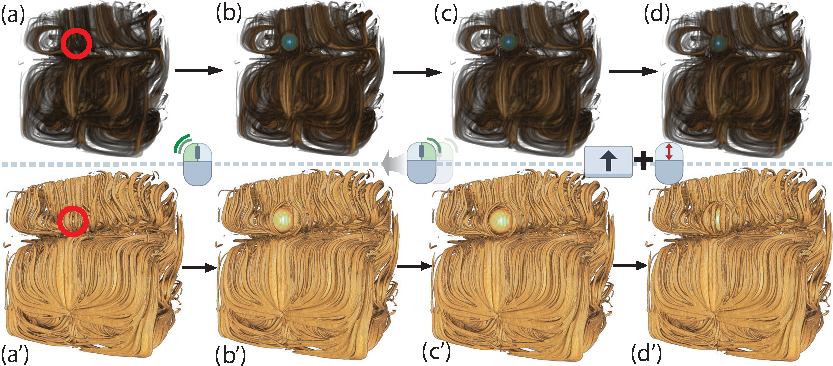
\includegraphics [width=0.95\textwidth]{images/stream_lens.eps}
\vspace{-0.15cm}
\caption{Flow volume exploration with two different opacity transfer functions (top and bottom rows). In viewpoint (a), we notice a small high-density spherical item. (b) We apply the lens at that location (double click). (c) The directions of rays in the lens are changed to see the whole target in the lens (right click + mouse drag change direction). (d) The lens is gradually closed while keeping the focus area magnified (shift + scroll).}
\vspace{-0.15cm}
\label{f:stream_lens}
\end{figure*}

\subsection{Chest scan: A hard to see tumor}
\label{sec:chest}
%
In our third use-case, we consider a contrast chest CT scan ($512 \times 512 \times 110$ voxels) of an elderly patient with a sizeable lung tumor. The tumor was detected in a CT scan performed after the patient reported acute chest pain. Typical examination of these scans by the pulmonologist and radiologist in charge involves slice-based views. Figures~\ref{f:slicer}a-c and \ref{f:slicer}d-f show two such slice sets (axial, coronal, and sagittal views), produced using typical lung, respectively mediastinal, contrast presets. Although the tumor is visible in all these views, its exact shape, morphology, and connection to the lung walls are hard to assess. Finding such details on the tumor is essential, explained the doctors in charge, to determine the TNM score and also planning treatment. Using standard DVR makes the tumor and its 3D position partially visible (\autoref{f:slicer}f). Yet, occlusion from the rib cage and other tissues is still present. Using both TF presets and manually changing the TFs in the 3D Slicer tool\,\cite{slicer} used to create the DVR could not help de-occluding the tumor without making it partly transparent. The slice images in \autoref{f:slicer}a-f confirm this by showing that the gray values for the tumor and surrounding skin-and-muscle tissue are very similar. This is due to the fact that the tumor had grown rapidly and started necrotizing, which filled it with fluids, making its density very similar to that of the obstructing (skin and muscle) tissue, explained the pulmonologist. Hence, one cannot remove such occluding tissue in a classical DVR setting by opacity TF manipulation without also removing the tumor. This makes examining this specific tumor harder than for regular cases.

\begin{figure}[htb]
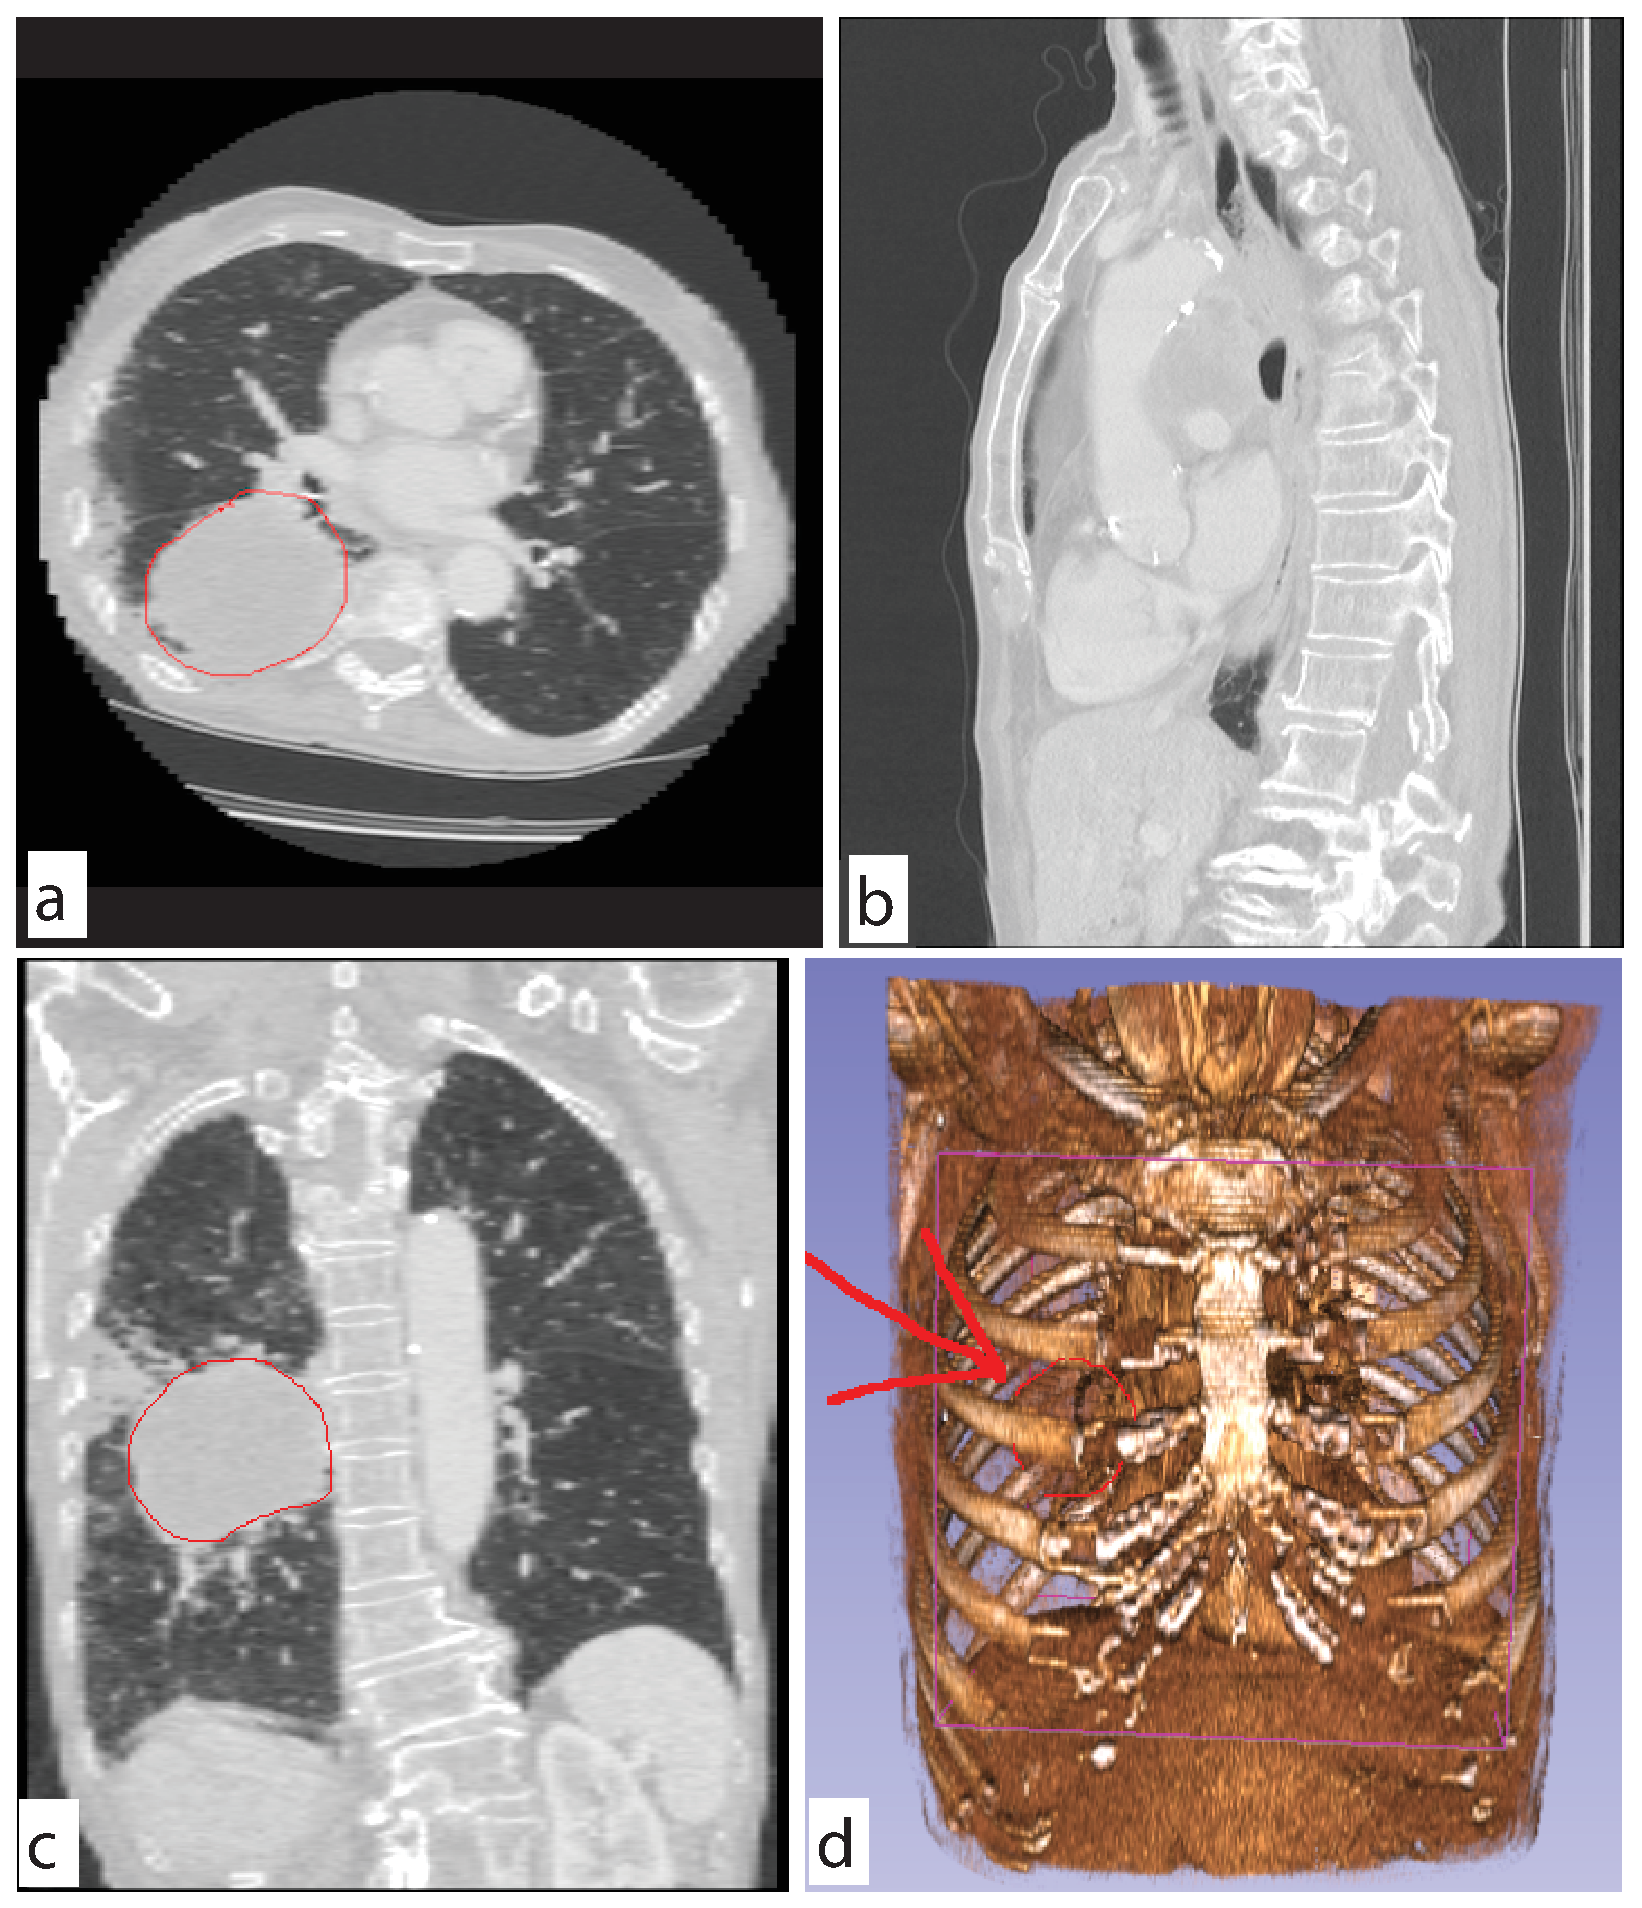
\includegraphics [width=0.48\textwidth]{images/slicer.eps}
\caption{Lung tumor visualization using slices (a-c) and standard DVR (d). Annotations are manually added by the examiner to delineate the tumor location. Images constructed using the 3D Slicer tool\,\cite{slicer}.}
\label{f:slicer}
\end{figure}

We next used our lens to examine the tumor. \autoref{f:params} shows several sample snapshots. We see that the tumor is significantly more visible when using the lens than when using standard DVR (\autoref{f:slicer}d), both in terms of removing the occluding tissue and in terms of the tumor's opacity -- compare the inset in \autoref{f:slicer}d with the images in \autoref{f:params}. Secondly, relighting the tumor from various directions allows one to see small-scale morphological details such as the tumor's surface shape and its connection via protuberances and veins with the lung walls.

We asked the two medical specialists (pulmonologist and radiologist) in charge to state the potential advantages and/or limitations of our lens as compared to standard slicing and DVR techniques, after a 20-minute usage of the tool. 
Both specialists have over 10 years of medical experience in treating lung cancer, and routinely use several slicing and DVR tools. They work in a private hospital in Belgium and are not actively associated to medical imaging research. Our identities were hidden from them during the lens evaluation. The provided input can be summarized as follows: The occlusion-free lens is definitely easier and faster to use than classical DVR and/or slicing techniques. It is especially more effective than these to get a quick, first impression of a deep buried anatomical detail. Changing the lens' parameters by direct interaction is as simple as changing window/level functions in a typical slice-based tool, and is definitely simpler than tuning typical DVR parameters to obtain similar results. This `entices' the user to explore, which is a good aspect. The fact that the lens minimizes viewpoint change (volume rotation), \emph{i.e.}, after a suitable viewpoint was found from which a (small) part of the target is visible, one doesn't need to change this viewpoint, is a strong feature, as 3D viewpoint changes are disruptive and cost time. This is important in a cost-aware environment where specialists have very limited time (about 20 minutes) to assess a CT scan. However, the lens should not \emph{replace} classical slice-based exploration, which shows small-scale details better. In the context of the current dataset (Fig.~\ref{f:slicer}), the lens was useful to both confirm the TNM score (T3 grade tumor, 6.5 cm in size) found via the 2D slices, but much more so for understanding how and where the tumor is connected to surrounding tissue, which is very hard to do using only 2D slices.

\begin{figure}
\centering
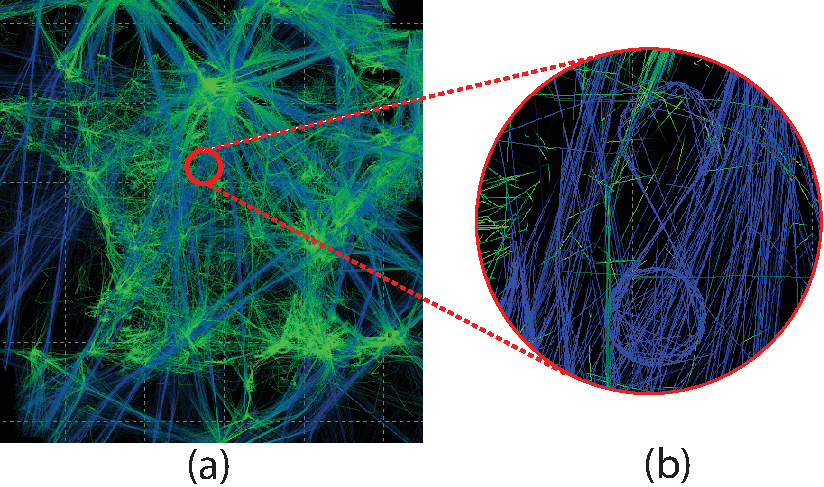
\includegraphics [width=0.48\textwidth]{images/aircraft.pdf}
\vspace{-0.15cm}
\caption{Visualizing one day of aircraft trajectories over France\,\cite{hurter2009fromdady}. (a) Overview of all trails. (b) Zoom, filtering, and color mapping techniques are used to highlight an outlier trajectory of an aircraft performing an eight-shaped loop. Revealing this outlier costs significant user effort.}
\label{f:fromdady}
\vspace{-0.15cm}
\end{figure}


\subsection{Aircraft trajectories: Outliers in the French sky}
\label{sec:atc}
%
%
We next consider a task from air traffic planning -- detecting and studying outliers in large-scale datasets containing tens of thousands of 3D (latitude, longitude, height) trails of aircraft over a given spatio-temporal region\,\cite{hurter2014interactive}. Such datasets are typically viewed using 2D (latitude, longitude) plots where opacity encodes the spatial density of flights -- see \autoref{f:fromdady}a, which shows one day of recorded aircraft trajectories over the French air space. \autoref{f:fromdady}(b) shows a detail zoom-in, where we can see an abnormal -- that is, far from straight or slightly curved -- aircraft trail: A tanker aircraft performed an eight-shaped loop as it was waiting to refuel other aircraft. Revealing such patterns using 2D techniques, \emph{e.g.} \cite{hurter2009fromdady}, is very hard. In particular, it is hard to de-occlude these patterns from the overall context of criss-crossing aircraft trails, even when one knows their 2D spatial location.

Our lens can help for this task, as follows. We first convert the set of 3D trails to a $500^3$ density volume, using KDE as for the streamline use-case (Sec.~\ref{sec:flow}). Examining this volume via standard DVR shows an outlier trail at some point in space, see curved patterns in \autoref{f:aircraft_lens}a. Activating the lens on this area and interactively tuning the target depth $t_{min}$ (since we don't know the trail's height) beings the outlier trajectory in focus and pushes away occluding trails (\autoref{f:aircraft_lens}a). Like in the other examples presented so far, we can quickly change the magnification factor and view direction to better study this trail in context (\autoref{f:aircraft_lens}b-d). From these images, we easily see that the outlier trail has an eight shape. Revealing this outlier trail using standard 2D visualization techniques\,\cite{hurter2009fromdady} costs several minutes. Doing the same using our lens costs under one minute. Also, comparing Figs.~\ref{f:fromdady}b and~\ref{f:aircraft_lens}b-d, we argue that the eight-shape of the outlier trail is much more prominent, and thus recognizable, in the latter images (made using our lens) than in the former ones. Last but not least, the 3D DVR approach that our lens enhances explicitly encodes flight height information, so our lens can use it by interactively tuning the depth value $t_{min}$ where the lens is focused. This cannot be done with 2D techniques which ignore the depth dimension.

We validated our findings with an air traffic data scientist with more than 10 year experience in air traffic control and planing. She confirmed that this specific eight-shape trail in \autoref{f:fromdady}(b) is an actual aircraft which performed waiting loops and acted as a fuel supplier for military aircraft. Other comments included the following: Compared to standard 2D visualization techniques, our tool makes detecting outliers easy since there is no need for complex manipulation to reveal such outlier trails. Also, the user does not have to deal with color and alpha mapping parameter-tuning to make specific outliers emerge. Separately, trail visualization easily creates many occlusions leading to either fully opaque areas or too much local overlap, both which hinder seeing and examining specific trails. Our lens does help such cases by distorting the space to locally remove such occlusions. All in all, in the studied dataset (\autoref{f:fromdady}), the lens was specifically useful since, for high transparency, one would not detect the outlier trail, while for low transparency, one would get a hint of the outlier's existence, but not see it in detail due to too much occlusion; the lens allows using low transparency, but removes the clutter caused by it to reveal the outlier.


\begin{figure*}[htbp]
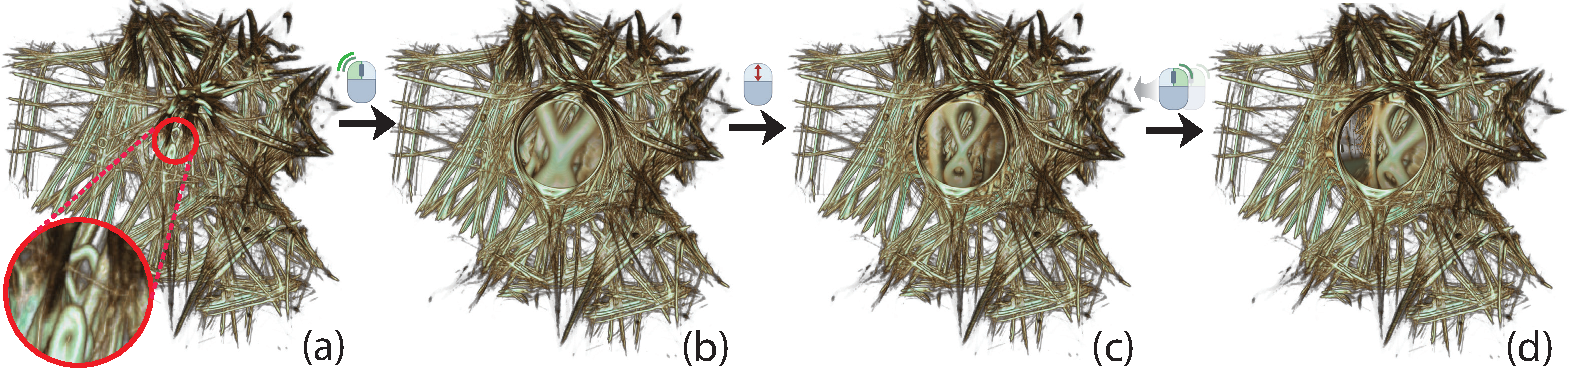
\includegraphics [width=0.98\textwidth]{images/aircraft_lens.pdf}
\caption{Inspecting an abnormal aircraft trail. (a) The abnormal trail is spotted in an all-trails view as it is highly curved while all other trails are relatively straight. Activating the lens at the outlier location (b) and changing the magnification factor (c) reveals the trail's eight-shape. (d) Rotating the viewpoint provides spatial insight on the embedding of the outlier in the surrounding trails.}
\label{f:aircraft_lens}
\end{figure*}
%

\subsection{Brain fibers: Uncluttering the bridge}
\label{sec:dti}
%
Our last use-case considers the exploration of fiber tracts visualized as streamlines of the major eigenvector of a diffusion tensor imaging (DTI) field. Such datasets have a spatially complex structure which makes them hard to explore\,\cite{assaf08}. In particular, fiber tracts are spread volumetrically over the entire extent of the brain, and create tangled patterns inside which it is hard to see much. DVR techniques are often used to render such tracts, one of the advantages being that close fibers get visually `merged' to reveal spatially coherent structures, an effect which is not possible when fibers are rendered as polylines. However, DVR methods also create more occlusion, thus difficulties in seeing structures deep within the volume.

We consider an $128 \times 128 \times 51$ DTI volume (same dataset as in\,\cite{everts15}). We traced 150352 fibers seeded in, and going over, regions of high fractional anisotropy in this volume. We filtered out fibers shorter than 2mm, yielding a total of 120593 fibers to display (6.4M sample points). Next, we converted this fiber-set to a $512^3$ density volume, using KDE with a 3D isotropic kernel of radius 15 voxels, like for the streamline use-case (Sec.~\ref{sec:flow}). Figure~\ref{fig:dti}a shows the result, rendered with DVR, with opacity function mapping the fiber density. While terminal fibers are well visible, we cannot see anything inside the volume. Activating the lens in the middle of the volume opens a hole through which a small part of the \emph{corpus callosum}, the fiber bundle wrapping the bridge that connects the two hemispheres, becomes visible. By slightly decreasing opacity (Fig.~\ref{fig:dti}c), the \emph{corpus callosum} gets clearly visible, appearing as a compact structure, due to the KDE blending of neighbor fibers. Obtaining such a view of the \emph{corpus callosum} using only DVR would be very hard, since transfer functions would either render separated (non-merged) fibers, or else make the fibers surrounding the structure of interest too thick and occluding. 

This scenario has a main difference compared to all previous ones. In all earlier cases, the standard DVR of the data (that is, without the lens) showed us a partial small cue of the structure of interest within the volume, and we used the screen-space location of this structure as the focus point where to activate the lens. In this last scenario, there is no point in the original DVR image (Fig.~\ref{fig:dti}a) from which the \emph{corpus callosum} is even partially visible, due to the high opacity given by the used transfer function. Hence, the user can activate the lens at \emph{any} desired point to peek inside, and towards the center of, the volume. Gven the nature of the data, the structure of interest is quite easily visible from most such viewpoints (see lens inset in Fig.~\ref{fig:dti}b). Once its presence is revealed, the user can next adjust the viewpoint and/or the opacity transfer function to get an optimal view on the target, such as the one shown in Fig.~\ref{fig:dti}c. Summarizing, we can use our lens also in cases when no partial view of a target is available. 

\begin{figure}[htbp!]
\centering
\includegraphics [width=0.45\textwidth]{images/dti.eps}
\caption{Revealing the \emph{corpus callosum} in a DVR of a set of DTI tracts.}
\label{fig:dti}
\end{figure}


%
